\newpage
\section{Общие сведения о системе}
\subsection{Запуск приложения}

\tmis~работает через Web-интерфейс и не требует установки на клиентской рабочей станции никакого дополнительного программного обеспечения. Единственным обязательным условием является наличие установленного Web-браузера, который, как правило, включен по умолчанию в состав любой операционной системы.

Для запуска приложения следует использовать соответствующий ярлык на рабочем столе. При его отсутствии можно запустить Web-браузер и в адресной строке ввести адрес сервера, через который осуществляется доступ к системе. Адрес сервера можно уточнить у администратора системы. 

\subsection{Авторизация пользователей}

\subsection{Вход в систему}

После запуска \tmis , необходимо выполнить вход в систему, используя персональный идентификатор пользователя и пароль. Процедура входа в систему называется \dm{авторизацией}. \label{auth}

Перед первым входом в систему необходимо получить персональный идентификатор пользователя (логин) и пароль у администратора системы.

\begin{vnim}
 Персональный идентификатор и пароль предназначены для индивидуального доступа в систему. Никогда не сообщайте их третьим лицам!
\end{vnim}
 
Следует ввести идентификатор пользователя и пароль в соответствующие поля на странице входа в систему (Рисунок \ref{img_gen_login}) и нажать кнопку \btn{Войти}.

\begin{figure}[!ht]\centering
 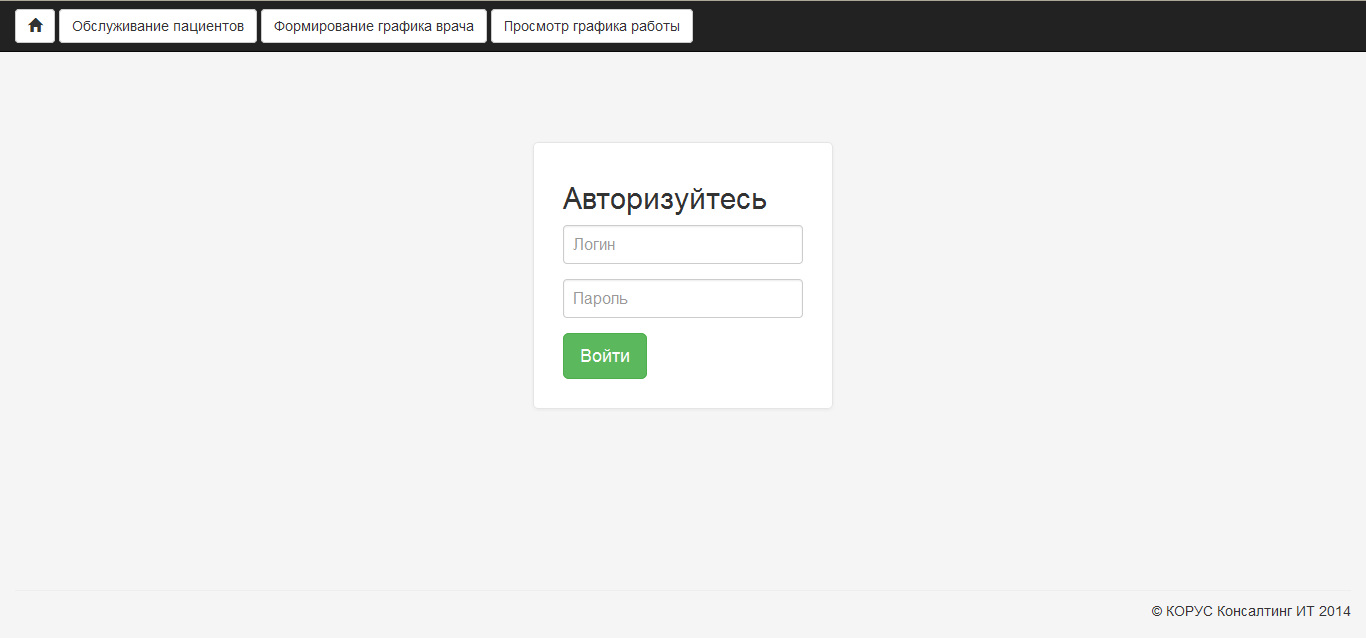
\includegraphics[width = 1\textwidth ,keepaspectratio]{gen_login}
 \caption{Страница авторизации}
 \label{img_gen_login}
\end{figure} 

Если логин и пароль пользователя введены верно, то будет осуществлен вход в систему. Если у пользователя имеется несколько ролей в системе, то дополнительно откроется страница выбора роли пользователя (Рисунок \ref{img_gen_rol}). При наличии единственной роли сразу будет осуществлен переход на главную страницу системы (Рисунок \ref{img_gen_main}).

\begin{figure}[!ht]\centering
 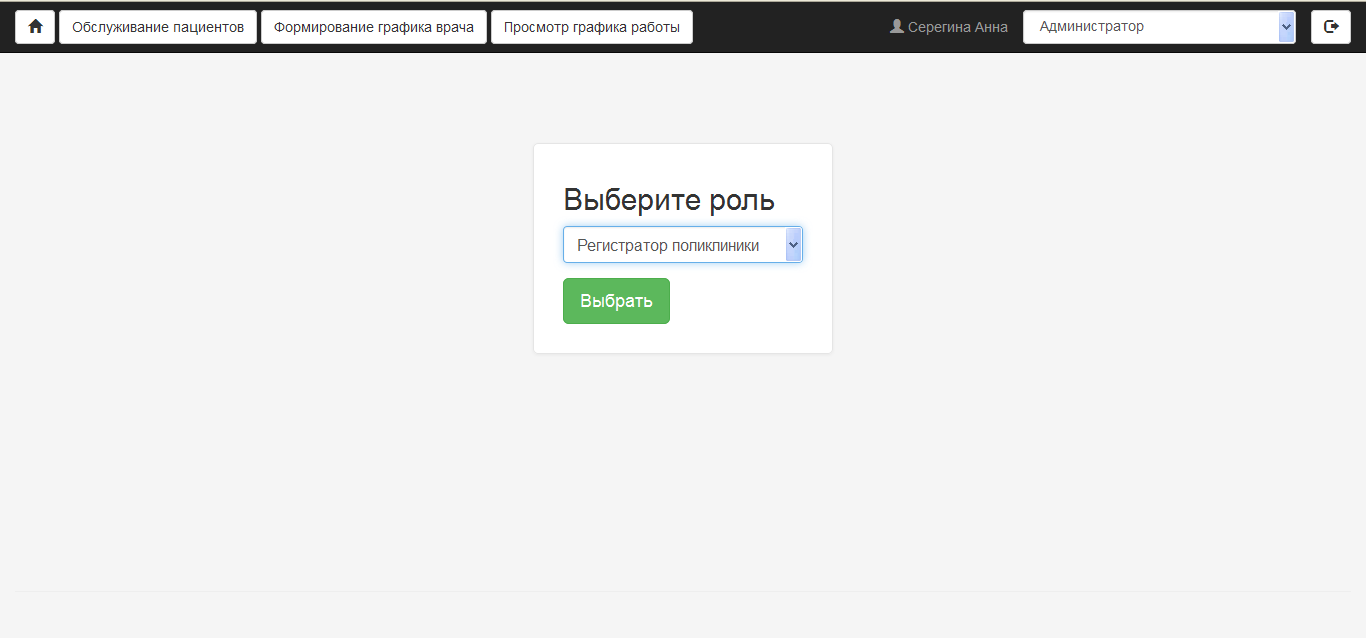
\includegraphics[width = 1\textwidth ,keepaspectratio]{gen_rol}
 \caption{Страница выбора роли пользователя}
 \label{img_gen_rol}
\end{figure} 

\begin{figure}[!ht]\centering
 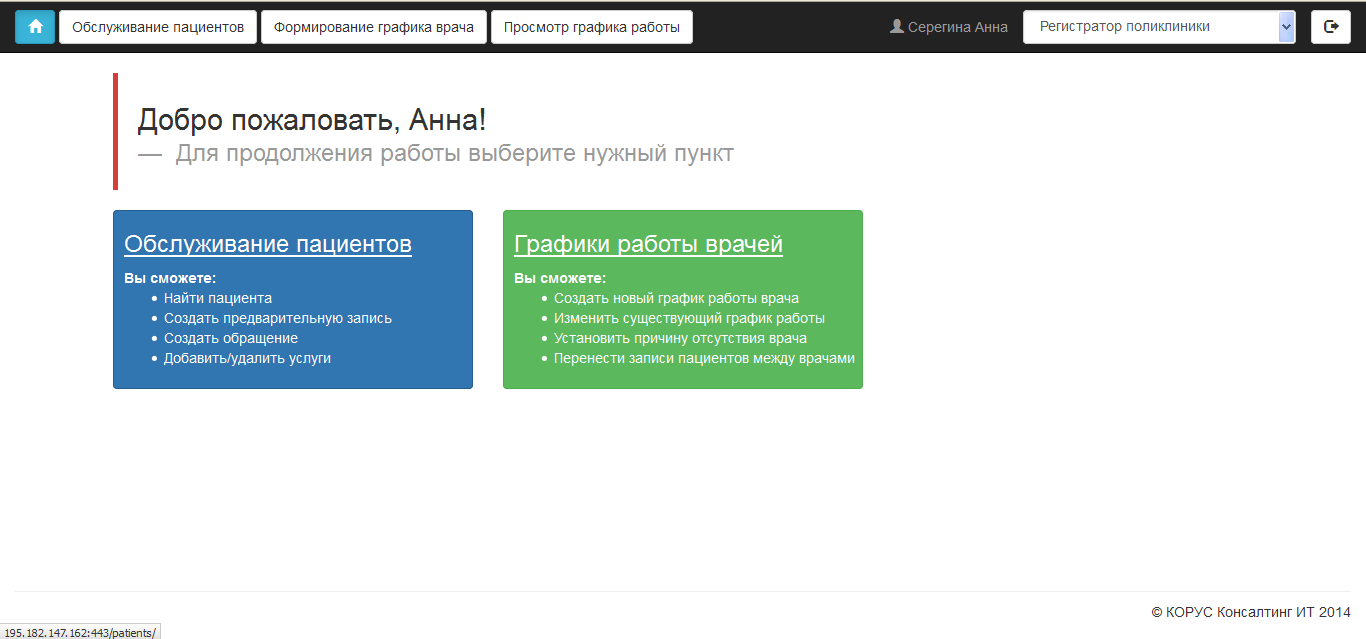
\includegraphics[width = 1\textwidth ,keepaspectratio]{gen_main}
 \caption{Главная страница системы}
 \label{img_gen_main}
\end{figure} 

Если в процессе авторизации возникла какая-либо ошибка, то вход в систему не будет осуществлен, а над полем для ввода логина появится сообщение об ошибке (Рисунок \ref{img_gen_lfail}).

В случае возникновения ошибки <<Неверная пара логин/пароль>> необходимо:
\begin{enumerate}
 \item Проверить правильность введенного идентификатора пользователя;
 \item Проверить правильность введенного адреса для подключения (если вводился вручную);
 \item Проверить язык ввода;
 \item Проверить состояние клавиши \keys{CapsLock} на клавиатуре и выключить ее при необходимости;
 \item Если в пароле присутствуют цифры, проверить состояние клавиши \keys{NumLock}, включить ее при необходимости;
 \item Повторить попытку авторизации.
\end{enumerate}
 
Если проблема не была решена, нужно обратиться к администратору системы для проверки идентификационных данных.

\begin{figure}[!ht]\centering
 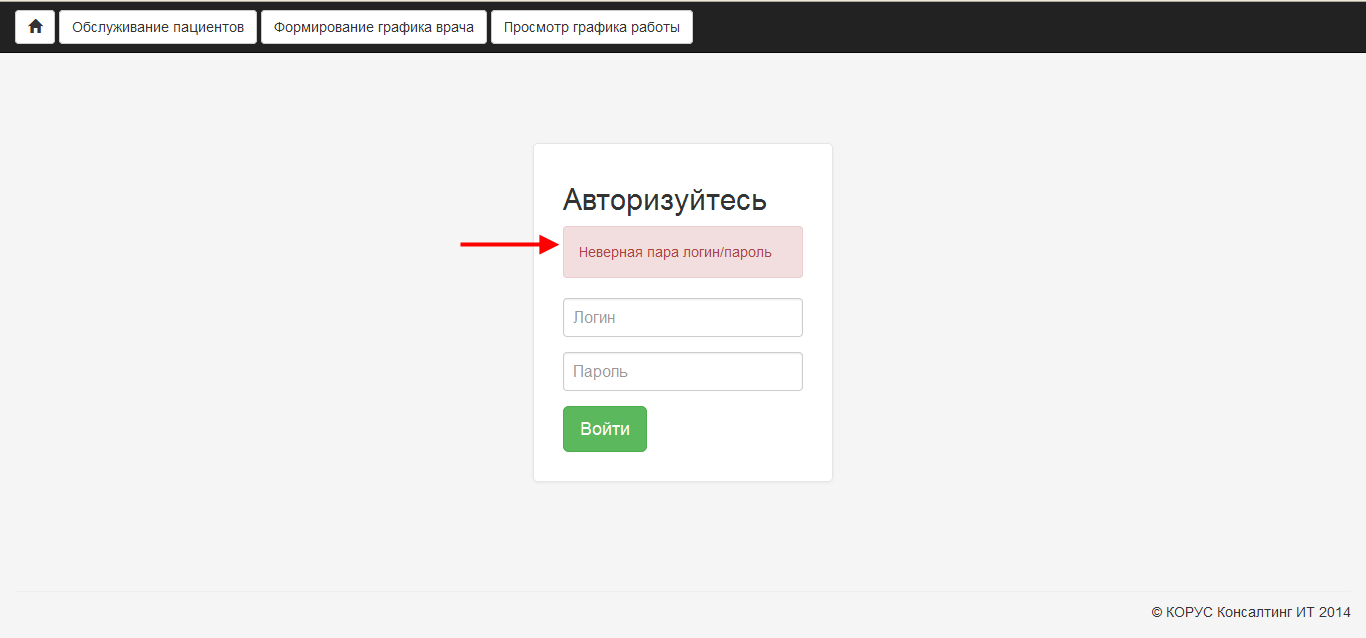
\includegraphics[width = 1\textwidth ,keepaspectratio]{gen_lfail}
 \caption{Ошибка авторизации}
 \label{img_gen_lfail}
\end{figure} 

\subsection{Завершение работы}

После окончания работы, необходимо выйти из системы. Для этого нужно нажать кнопку 
\includegraphics[scale=0.6]{exit} в правом верхнем углу страницы. Будет осуществлен выход из системы и возврат на страницу авторизации. Если требуется войти в систему под другим именем пользователя, следует пройти процедуру авторизации с новыми идентификационными данными. Если работа с системой завершена, можно закрыть Web-браузер, нажав на кнопку \btn{x} в правом верхнем углу окна или выбрав в главном меню пункт \mm{Файл \str Выход}.

\subsection{Основные принципы работы}

Вся работа в системе производится в окне Web-браузера. В верхней части каждой страницы находится панель управления (Рисунок \ref{img_gen_main}).

В левой ее части находятся список основных доступных операций пользователя. При нажатии на кнопку с названием операции осуществляется переход на страницу работы с соответствующей функцией системы. При нажатии на кнопку 
\includegraphics[scale=0.6]{home}, расположенную в левом верхнем углу страницы, выполняется переход на главную страницу системы.

В правой части панели управления указано имя пользователя, под которым был осуществлен вход в систему и текущая роль пользователя. При наличии у пользователя нескольких ролей можно быстро сменить ее, выбрав другую роль из раскрывающегося списка на панели управления. В правом верхнем углу расположена кнопка 
\includegraphics[scale=0.6]{exit}, позволяющая выйти из системы.

\begin{prim}
 После авторизации в системе возможно одновременное открытие нескольких страниц системы. Страницы могут быть открыты в отдельных окнах или вкладках. Для открытия страницы в новой вкладке или новом окне можно воспользоваться контекстным меню или колесом прокрутки мыши.
\end{prim}

